% Generated by build/sync_schwartz_qft.py from committed sources only.
% Source repository: https://github.com/Luca-Yucheng-Jin/schwartz-qft-solutions
% Source commit: ffb03aac5f7e5c8fbc1bc01082c2a54335364148
\documentclass[a4paper,11pt]{article}
\usepackage{amsmath,amssymb,bm,graphicx,slashed,tikz,tikz-feynman}
\DeclareMathOperator{\Tr}{Tr}
\newenvironment{solution}{\par\medskip\noindent\textbf{Solution.}\par\smallskip}{\par\medskip}
\newenvironment{problemparts}{\begin{enumerate}\renewcommand{\labelenumi}{(\alph{enumi})}}{\end{enumerate}}
\title{Completed Solutions to Schwartz's \textit{Quantum Field Theory and the Standard Model}}
\author{Luca Yucheng Jin}
\begin{document}
\maketitle

\subsection[Problem 29.1: Higgs production at LEP]{Problem 29.1: Higgs Production at LEP}

The dominant production mechanism for Higgs bosons at LEP was
$e^+e^-\to ZH$. Calculate the total cross section for this process at
tree-level in the Standard Model. How many $100\,\mathrm{GeV}$ Higgs bosons
would there have been when LEP ran at $206\,\mathrm{GeV}$?

\begin{solution}
In this question, the relevant sector of the electroweak Lagrangian at
tree-level is given by
\begin{equation}
    \mathcal{L} = - \frac{1}{2}h(\square  + m_h^2)h
    + \bar{\psi}(i\slashed{\partial} -m_e)\psi
    + \frac{1}{v}m_Z^2Z_\mu Z^\mu h
    + \frac{e}{\sin\theta_w\cos\theta_w}Z_\mu
    (J^{3\mu}-\sin^2\theta_wJ^{\mathrm{EM}\mu}),
\end{equation}
where $v = 2\frac{m_W}{e}\sin\theta_w$,
$J_\mu ^{\mathrm {EM}} = -\bar\psi\gamma_\mu \psi$ and
\begin{equation}
    J_\mu^3 = \bar \psi^L \gamma_\mu T^3 \psi^L
    = \bar\psi P_R \gamma_\mu T^3P_L\psi
    = \bar \psi \gamma_\mu P_L T^3P_L \psi
    = \bar \psi \gamma_\mu T^3P_L \psi
    = -\frac{1}{2}\bar\psi\gamma_\mu P_L\psi,
\end{equation}
where we have used $[P_L,T^3] =0$, $T^3\psi^L = -\frac{1}{2}\psi^L$
and $P_L^2 = P_L$. Therefore, the $ZZh$ interaction is given by
\begin{equation}
\begin{tikzpicture}[baseline=(v.center)]
  \begin{feynman}
    \vertex (v) at (0,0);
    \vertex (h)  at (0,1.0)       {$h$};
    \vertex (z1) at (-1.4,-0.8)   {$Z^\mu$};
    \vertex (z2) at (1.4,-0.8)    {$Z^\nu$};

    \diagram*{
      (h)  -- [scalar, thick] (v),
      (z1) -- [boson, thick]  (v),
      (z2) -- [boson, thick]  (v),
    };
  \end{feynman}
\end{tikzpicture}
\quad = \quad
i\frac{e}{\sin\theta_w\cos^2\theta_w}m_Wg^{\mu\nu}.
\label{eq:ZZh-interaction}
\end{equation}
The $eeZ$ interaction is given by
\begin{equation}
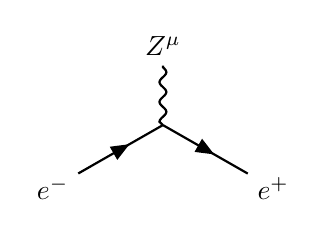
\begin{tikzpicture}[baseline=(v.center)]
  \begin{feynman}
    \vertex (v) at (0,0);
    \vertex (z)  at (0,1.0)       {$Z^\mu$};
    \vertex (em) at (-1.4,-0.8)   {$e^-$};
    \vertex (ep) at (1.4,-0.8)    {$e^+$};

    \diagram*{
      (z)  -- [boson, thick]   (v),
      (em) -- [fermion, thick] (v),
      (v)  -- [fermion, thick] (ep),
    };
  \end{feynman}
\end{tikzpicture}
\quad = \quad
i\frac{e}{\sin\theta_w\cos\theta_w}
\gamma^\mu
\left(
-\frac{1-\gamma^5}{4}
+\sin^2\theta_w
\right).
\label{eq:eeZ-interaction}
\end{equation}
The only diagram we are concerned with at tree-level is
\begin{equation}
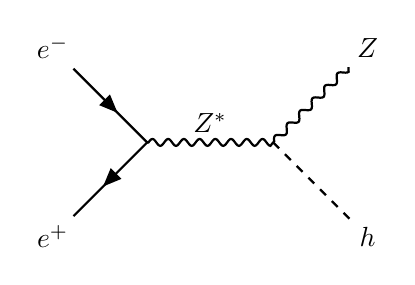
\begin{tikzpicture}[baseline=(v1.center)]
  \begin{feynman}
    \vertex (v1) at (-0.8,0);
    \vertex (v2) at (0.8,0);

    \vertex (em) at (-2.0,1.2)  {$e^-$};
    \vertex (ep) at (-2.0,-1.2) {$e^+$};

    \vertex (z) at (2.0,1.2)  {$Z$};
    \vertex (h) at (2.0,-1.2) {$h$};

    \diagram*{
      (em) -- [fermion, thick] (v1),
      (v1) -- [fermion, thick] (ep),
      (v1) -- [boson, thick, edge label=$Z^*$] (v2),
      (v2) -- [boson, thick] (z),
      (v2) -- [scalar, thick] (h),
    };
  \end{feynman}
\end{tikzpicture}
\quad = \quad i\mathcal{M}.
\label{eq:ee-to-Zh-tree}
\end{equation}
We can read off from the Feynman rules we just wrote down that
\begin{equation}
\begin{aligned}
        i\mathcal{M} &=
        \left(i\frac{e}{\sin\theta_w\cos\theta_w}\right)
        \left(i\frac{em_W}{\sin\theta_w\cos^2\theta_w}\right)\\
        &\quad \times\left[\bar v(p_2)\gamma^\mu
        \left(-\frac{1-\gamma^5}{4}+\sin^2\theta_w\right)u(p_1)\right]
        \frac{-ig_{\mu\nu}}{s-m_Z^2}g^{\nu\rho}
        \epsilon^*_\rho(p_3)\\
        &= \frac{ie^2m_W}{\sin^2\theta_w\cos^3\theta_w}
        \frac{1}{s-m_Z^2}\epsilon_\mu^*(p_3)
        \left[\bar v(p_2)\gamma^\mu
        \left(-\frac{1-\gamma^5}{4}+\sin^2\theta_w\right)u(p_1)\right].
\end{aligned}
\end{equation}
Here the longitudinal part of the internal $Z$ propagator vanishes by current
conservation when $m_e=0$. Taking the modulus square and summing over the
external spins and polarisations, we find
\begin{equation}
\begin{aligned}
    \sum_{\mathrm{spins/pols.}}|\mathcal{M}|^2
    &= \left(\frac{e^2m_W}{\sin^2\theta_w\cos^3\theta_w}\right)^2
    \frac{1}{(s-m_Z^2)^2}
    \sum_{\mathrm{pols.}}\epsilon_\mu^*(p_3)\epsilon_\nu(p_3)\\
    &\quad\times\Tr\left[\slashed{p}_2\gamma^\mu
    \left(-\frac{1-\gamma^5}{4}+\sin^2\theta_w\right)
    \slashed{p}_1\gamma^\nu
    \left(-\frac{1-\gamma^5}{4}+\sin^2\theta_w\right)\right],
\end{aligned}
\end{equation}
where we have taken $m_e =0$. The symmetric part of the trace over spinors is
\begin{equation}
    \left(4\sin^4\theta_w-2\sin^2\theta_w+\frac{1}{2}\right)
    \left(p_1^\mu p_2^\nu + p_1^\nu p_2^\mu
    -p_1\cdot p_2 g^{\mu\nu}\right).
\end{equation}
The antisymmetric part does not contribute when contracted with the
polarisation sum, which is given by
\begin{equation}
    \sum_{\mathrm{pols.}}\epsilon_\mu^*(p_3)\epsilon_\nu(p_3)
    = -g_{\mu\nu}+ \frac{p_{3\mu}p_{3\nu}}{m_Z^2}.
\end{equation}
Putting them together, we find
\begin{equation}
\begin{aligned}
    \sum_{\mathrm{spins/pols.}}|\mathcal{M}|^2
    &= \left(\frac{e^2m_W}{\sin^2\theta_w\cos^3\theta_w}\right)^2
    \frac{4\sin^4\theta_w-2\sin^2\theta_w+\frac{1}{2}}
    {(s-m_Z^2)^2}\\
    &\quad\times\left(2p_1\cdot p_2
    + \frac{2(p_1\cdot p_3)(p_2\cdot p_3)}{m_Z^2}
    - \frac{(p_1\cdot p_2)p_3^2}{m_Z^2}\right).
\end{aligned}
\end{equation}
To compute the cross-section, we need to average over the initial spins, which
is to multiply by a factor of $1/4$. In the centre-of-mass frame, we have
\begin{equation}
\begin{gathered}
    p_3^2=m_Z^2,\qquad p_1\cdot p_2=\frac{s}{2},\qquad
    |\mathbf{k}|=\frac{\sqrt{s}}{2},\\
    (p_1\cdot p_3)(p_2\cdot p_3)
    =\frac{s}{4}\left(E_Z^2-|\mathbf{p}|^2\cos^2\theta\right),
    \qquad E_Z=\sqrt{|\mathbf{p}|^2+m_Z^2},
\end{gathered}
\end{equation}
where $\mathbf{k}$ is the momentum of the incoming electron and positron and
$\mathbf{p}$ is the momentum of the outgoing $Z$ and Higgs bosons. Hence,
\begin{equation}
\begin{aligned}
    \sum_{\mathrm{spins/pols.}}|\mathcal{M}|^2
    &=\left(\frac{e^2m_W}{\sin^2\theta_w\cos^3\theta_w}\right)^2
    \frac{s\left(4\sin^4\theta_w-2\sin^2\theta_w+\frac{1}{2}\right)}
    {(s-m_Z^2)^2}\\
    &\quad\times\left[1+
    \frac{\left[s-(m_Z+m_h)^2\right]\left[s-(m_Z-m_h)^2\right]}
    {8sm_Z^2}\sin^2\theta\right].
\end{aligned}
\end{equation}
The magnitude of the outgoing three-momentum is
\begin{equation}
    |\mathbf{p}|=
    \frac{\sqrt{\left[s-(m_Z+m_h)^2\right]
    \left[s-(m_Z-m_h)^2\right]}}{2\sqrt{s}},
\end{equation}
and therefore
\begin{equation}
    \frac{|\mathbf{p}|}{|\mathbf{k}|}
    =\frac{\sqrt{\left[s-(m_Z+m_h)^2\right]
    \left[s-(m_Z-m_h)^2\right]}}{s}.
\end{equation}
It follows that
\begin{equation}
\begin{aligned}
    \frac{d\sigma}{d\Omega}
    &=\frac{1}{64\pi^2s}\frac{|\mathbf{p}|}{|\mathbf{k}|}
    \frac{1}{4}\sum_{\mathrm{spins/pols.}}|\mathcal{M}|^2\\
    &=\frac{\alpha^2m_W^2
    \left(4\sin^4\theta_w-2\sin^2\theta_w+\frac{1}{2}\right)}
    {16\sin^4\theta_w\cos^6\theta_w(s-m_Z^2)^2}
    \frac{\sqrt{\left[s-(m_Z+m_h)^2\right]
    \left[s-(m_Z-m_h)^2\right]}}{s}\\
    &\quad\times\left[1+
    \frac{\left[s-(m_Z+m_h)^2\right]\left[s-(m_Z-m_h)^2\right]}
    {8sm_Z^2}\sin^2\theta\right].
\end{aligned}
\end{equation}
Using $\int d\Omega=4\pi$ and
$\int d\Omega\,\sin^2\theta=8\pi/3$, the total cross section is
\begin{equation}
\begin{aligned}
    \sigma(e^+e^-\to Zh)
    &=\frac{\pi\alpha^2m_W^2
    \left(4\sin^4\theta_w-2\sin^2\theta_w+\frac{1}{2}\right)}
    {4\sin^4\theta_w\cos^6\theta_w(s-m_Z^2)^2}
    \frac{\sqrt{\left[s-(m_Z+m_h)^2\right]
    \left[s-(m_Z-m_h)^2\right]}}{s}\\
    &\quad\times\left[1+
    \frac{\left[s-(m_Z+m_h)^2\right]\left[s-(m_Z-m_h)^2\right]}
    {12sm_Z^2}\right].
\end{aligned}
\end{equation}
For the numerical estimate, we take
\begin{equation}
    \sqrt{s}=206\,\mathrm{GeV},\qquad
    m_h=100\,\mathrm{GeV},\qquad
    m_Z=91.2\,\mathrm{GeV},\qquad
    m_W=80.4\,\mathrm{GeV},
\end{equation}
together with
\begin{equation}
    \sin^2\theta_w=0.231,
    \qquad
    \alpha=\frac{1}{128}.
\end{equation}
Substituting these values into the total cross section gives
\begin{equation}
    \sigma(e^+e^-\to Zh)
    \simeq 1.09\times10^{-9}\,\mathrm{GeV}^{-2}.
\end{equation}
Using
\begin{equation}
    1\,\mathrm{GeV}^{-2}
    =3.894\times10^8\,\mathrm{pb},
\end{equation}
this becomes
\begin{equation}
    \sigma(e^+e^-\to Zh)\simeq0.42\,\mathrm{pb}.
\end{equation}
The four LEP experiments collected an integrated luminosity of approximately
$536\,\mathrm{pb}^{-1}$ at centre-of-mass energies of $206\,\mathrm{GeV}$
or higher. The expected number of produced Higgs bosons is therefore
\begin{equation}
    N=\sigma L_{\mathrm{int}}
    \simeq(0.42\,\mathrm{pb})(536\,\mathrm{pb}^{-1})
    \simeq 2.3\times10^2.
\end{equation}
Thus, approximately
\begin{equation}
    \boxed{N\simeq230}
\end{equation}
$100\,\mathrm{GeV}$ Higgs bosons would have been produced.
\end{solution}

\subsection[Problem 29.2: \texorpdfstring{$e^+e^-\to$ hadrons}{electron-positron to hadrons}]{Problem 29.2: Electron-Positron Annihilation into Hadrons}

$e^+e^-\to\text{hadrons}$ in the Standard Model.

\begin{enumerate}
  \item Calculate the rate for the total cross section
  $\sigma_{\mathrm{tot}}(e^+e^-\to\text{hadrons})$ in the Standard Model at
  tree-level including both $Z$-boson and photon contributions and their
  interference. The contribution using photons alone was calculated in
  Section~26.3.

  \item Calculate $\sigma_{\mathrm{tot}}$ at 1-loop.

  \item Plot the total cross section as a function of center-of-mass energy
  showing separately the photon contribution, the $Z$-boson contribution, and
  their sum. Plot also the sum ignoring interference between the $Z$-boson and
  photon contributions. When can interference be ignored?
\end{enumerate}

\begin{solution}
For the $e^+e^- \to \gamma^* \to \mathrm{hadrons}$, the relevant sector of the electroweak Lagrangian is
\begin{equation}
    \mathcal{L} = \bar \psi_e(i\slashed{\partial} - m_e)\psi_e + \sum_i\bar{\psi}_i(i\slashed{\partial} - m_i)\psi_i - e\bar \psi_e\slashed{A}\psi_e + e\sum_i Q_i\bar\psi_i \slashed{A}\psi_i,
\end{equation}
where $i$ denotes the up, down, strange, etc.
We can read off the scattering amplitude directly for a particular pair of quark and anti-quark, which is
\begin{equation}
    i\mathcal{M}_\gamma^i = (ie)^2Q_i[\bar v(p_2)\gamma^\mu u(p_1)]\frac{-i}{s}[\bar u_i(p_3)\gamma_\mu v_i(p_4)] = iQ_i\mathcal{M}_0,
\end{equation}
where $\mathcal{M}_0$ is the scattering amplitude of $e^-e^+\to \mu^-\mu^+$ at tree-level. Note that $Q_{u,c,t} = \frac{2}{3}$ and $Q_{d,s,b} = -\frac{1}{3}$.

The $Z$ boson coupling to a general quark field is given by
\begin{equation}
    \frac{ie}{\sin\theta_w\cos\theta_w}
    \gamma^\mu
    \left(
        T^3\frac{1-\gamma^5}{2}
        -Q_i\sin^2\theta_w
    \right)
    =
    \frac{ie}{4\sin\theta_w\cos\theta_w}
    \gamma^\mu
    \left(
        \xi_i\gamma^5
        -4Q_i\sin^2\theta_w
        -\xi_i
    \right),
\end{equation}
where
\begin{equation}
    \xi_i=
    \begin{cases}
        -1, & i=u,c,t,\\
        +1, & i=d,s,b.
    \end{cases}
\end{equation}
Defining
\begin{equation}
    a_i=4|Q_i|\sin^2\theta_w-1,
\end{equation}
the quark vertex can equivalently be written as
\begin{equation}
    \frac{ie}{4\sin\theta_w\cos\theta_w}
    \xi_i\gamma^\mu(\gamma^5+a_i).
\end{equation}
Therefore, the $Z$-exchange amplitude is
\begin{equation}
\begin{aligned}
    i\mathcal{M}_Z^i
    &=
    \left(
        \frac{ie}{4\sin\theta_w\cos\theta_w}
    \right)^2
    \left[
        \bar v(p_2)\gamma^\mu(\gamma^5+a)u(p_1)
    \right]
    \frac{-i}{s-m_Z^2}
    \left[
        \xi_i\bar u(p_3)\gamma_\mu(\gamma^5+a_i)v(p_4)
    \right],
\end{aligned}
\end{equation}
where
\begin{equation}
    a=4\sin^2\theta_w-1.
\end{equation}

The initial-state spin sum is
\begin{equation}
\begin{aligned}
    &\sum_{\mathrm{spins}}
    \left[
        \bar v(p_2)\gamma^\mu(\gamma^5+a)u(p_1)
    \right]
    \left[
        \bar u(p_1)\gamma^\nu(\gamma^5+a)v(p_2)
    \right]
    \\
    &\qquad =
    \Tr\left[
        \slashed{p}_2\gamma^\mu(\gamma^5+a)
        \slashed{p}_1\gamma^\nu(\gamma^5+a)
    \right]
    \\
    &\qquad =
    4(a^2+1)
    \left(
        p_1^\mu p_2^\nu
        +p_1^\nu p_2^\mu
        -p_1\cdot p_2\,\eta^{\mu\nu}
    \right)
    -8ia\,p_{1\alpha}p_{2\beta}
    \epsilon^{\alpha\mu\beta\nu}.
\end{aligned}
\end{equation}
Similarly, since $\xi_i^2=1$, the final-state spin sum is
\begin{equation}
\begin{aligned}
    &4(a_i^2+1)
    \left(
        p_{3\mu}p_{4\nu}
        +p_{3\nu}p_{4\mu}
        -p_3\cdot p_4\,\eta_{\mu\nu}
    \right)
    +8ia_i\,p_{3\alpha}p_{4\beta}
    \epsilon^{\alpha}{}_{\mu}{}^{\beta}{}_{\nu}.
\end{aligned}
\end{equation}
Thus,
\begin{equation}
\begin{aligned}
    \sum_{\mathrm{spins}}|\mathcal{M}_Z^i|^2
    &=
    \left(
        \frac{e}{4\sin\theta_w\cos\theta_w}
    \right)^4
    \frac{1}{(s-m_Z^2)^2}
    \\
    &\quad\times
    \Big[
        4(a^2+1)
        \left(
            p_1^\mu p_2^\nu
            +p_1^\nu p_2^\mu
            -p_1\cdot p_2\,\eta^{\mu\nu}
        \right)
        -8ia\,p_{1\alpha}p_{2\beta}
        \epsilon^{\alpha\mu\beta\nu}
    \Big]
    \\
    &\quad\times
    \Big[
        4(a_i^2+1)
        \left(
            p_{3\mu}p_{4\nu}
            +p_{3\nu}p_{4\mu}
            -p_3\cdot p_4\,\eta_{\mu\nu}
        \right)
        +8ia_i\,p_{3\alpha}p_{4\beta}
        \epsilon^{\alpha}{}_{\mu}{}^{\beta}{}_{\nu}
    \Big].
\end{aligned}
\end{equation}
The contraction between a symmetric tensor and an antisymmetric tensor
vanishes. Contracting the two symmetric terms and the two epsilon tensors
therefore gives
\begin{equation}
\begin{aligned}
    \sum_{\mathrm{spins}}|\mathcal{M}_Z^i|^2
    &=
    \frac{e^4}
    {8\sin^4\theta_w\cos^4\theta_w(s-m_Z^2)^2}
    \\
    &\quad\times
    \Big[
        \big((a^2+1)(a_i^2+1)-4aa_i\big)
        (p_1\cdot p_3)(p_2\cdot p_4)
        \\
        &\qquad\quad+
        \big((a^2+1)(a_i^2+1)+4aa_i\big)
        (p_1\cdot p_4)(p_2\cdot p_3)
    \Big].
\end{aligned}
\end{equation}
For massless external particles,
\begin{equation}
    p_1\cdot p_3=p_2\cdot p_4=-\frac{t}{2},
    \qquad
    p_1\cdot p_4=p_2\cdot p_3=-\frac{u}{2}.
\end{equation}
Hence,
\begin{equation}
\begin{aligned}
    \sum_{\mathrm{spins}}|\mathcal{M}_Z^i|^2
    &=
    \frac{e^4}
    {32\sin^4\theta_w\cos^4\theta_w(s-m_Z^2)^2}
    \\
    &\quad\times
    \left[
        \big((a^2+1)(a_i^2+1)-4aa_i\big)t^2
        +
        \big((a^2+1)(a_i^2+1)+4aa_i\big)u^2
    \right].
\end{aligned}
\end{equation}

For the photon--$Z$ interference term, the required mixed traces are
\begin{equation}
\begin{aligned}
    \Tr\left[
        \slashed{p}_2\gamma^\mu
        \slashed{p}_1\gamma^\nu(\gamma^5+a)
    \right]
    &=
    4a
    \left(
        p_1^\mu p_2^\nu
        +p_1^\nu p_2^\mu
        -p_1\cdot p_2\,\eta^{\mu\nu}
    \right)
    -4ip_{1\alpha}p_{2\beta}
    \epsilon^{\alpha\mu\beta\nu},
    \\
    \Tr\left[
        \slashed{p}_3\gamma_\mu
        \slashed{p}_4\gamma_\nu
        (\xi_i\gamma^5+\xi_i a_i)
    \right]
    &=
    4\xi_i a_i
    \left(
        p_{3\mu}p_{4\nu}
        +p_{3\nu}p_{4\mu}
        -p_3\cdot p_4\,\eta_{\mu\nu}
    \right)
    \\
    &\quad+
    4i\xi_i p_{3\alpha}p_{4\beta}
    \epsilon^{\alpha}{}_{\mu}{}^{\beta}{}_{\nu}.
\end{aligned}
\end{equation}
Therefore,
\begin{equation}
\begin{aligned}
    2\operatorname{Re}
    \sum_{\mathrm{spins}}
    \mathcal{M}_\gamma^i\mathcal{M}_Z^{i\dagger}
    &=
    \frac{e^4Q_i\xi_i}
    {\sin^2\theta_w\cos^2\theta_w\,
    s(s-m_Z^2)}
    \\
    &\quad\times
    \left[
        (aa_i-1)t^2+(aa_i+1)u^2
    \right].
\end{aligned}
\end{equation}

Putting the photon, $Z$, and interference contributions together and
averaging over the initial spins gives
\begin{equation}
\begin{aligned}
    \frac{1}{4}\sum_\mathrm{spin}{|\mathcal{M}^i|^2}
    &=
    \frac{e^4Q_i^2}{s^2}(t^2+u^2)
    \\
    &\quad+
    \frac{e^4}
    {128\sin^4\theta_w\cos^4\theta_w(s-m_Z^2)^2}
    \left[
        \big((a^2+1)(a_i^2+1)-4aa_i\big)t^2
        \right.
        \\
        &\hspace{7.3cm}\left.
        +
        \big((a^2+1)(a_i^2+1)+4aa_i\big)u^2
    \right]
    \\
    &\quad+
    \frac{e^4Q_i\xi_i}
    {4\sin^2\theta_w\cos^2\theta_w\,
    s(s-m_Z^2)}
    \left[
        (aa_i-1)t^2+(aa_i+1)u^2
    \right].
\end{aligned}
\end{equation}
Then, we sum over all flavours, which can be simplified as summing over the up and down flavour times three in our massless approximation. That is
\begin{equation}
    \frac{1}{4}\sum_i\sum_\mathrm{spin}{|\mathcal{M}^i|^2} = \frac{3}{4}\sum_\mathrm{spin}{|\mathcal{M}^u|^2 + |\mathcal{M}^d|^2}.
\end{equation}
Using
\begin{equation}
    Q_u=\frac{2}{3},
    \qquad
    Q_d=-\frac{1}{3},
    \qquad
    \xi_u=-1,
    \qquad
    \xi_d=1,
\end{equation}
and
\begin{equation}
    a_u=\frac{8}{3}\sin^2\theta_w-1,
    \qquad
    a_d=\frac{4}{3}\sin^2\theta_w-1,
\end{equation}
the required sums are
\begin{equation}
\begin{aligned}
    3\sum_{i=u,d}Q_i^2
    &=\frac{5}{3},\\
    3\sum_{i=u,d}
    \left[(a^2+1)(a_i^2+1)-4aa_i\right]
    &=
    \frac{32}{3}\sin^4\theta_w
    \left(
        40\sin^4\theta_w-56\sin^2\theta_w+23
    \right),\\
    3\sum_{i=u,d}
    \left[(a^2+1)(a_i^2+1)+4aa_i\right]
    &=
    \frac{16}{3}
    \left(
        80\sin^8\theta_w-112\sin^6\theta_w
        +118\sin^4\theta_w-54\sin^2\theta_w+9
    \right),\\
    3\sum_{i=u,d}Q_i\xi_i(aa_i-1)
    &=
    \frac{8}{3}\sin^2\theta_w
    \left(7-10\sin^2\theta_w\right),\\
    3\sum_{i=u,d}Q_i\xi_i(aa_i+1)
    &=
    -\frac{2}{3}
    \left(
        40\sin^4\theta_w-28\sin^2\theta_w+9
    \right).
\end{aligned}
\end{equation}
Therefore,
\begin{equation}
\begin{aligned}
    \frac{1}{4}\sum_i\sum_{\mathrm{spins}}|\mathcal M^i|^2
    &=
    \frac{10e^4}{3s^2}(t^2+u^2)
    \\
    &\quad+
    \frac{e^4}
    {24\sin^4\theta_w\cos^4\theta_w(s-m_Z^2)^2}
    \Big[
        2\sin^4\theta_w
        \left(
            40\sin^4\theta_w-56\sin^2\theta_w+23
        \right)t^2
    \\
    &\hspace{3.5cm}
        +
        \left(
            80\sin^8\theta_w-112\sin^6\theta_w
            +118\sin^4\theta_w-54\sin^2\theta_w+9
        \right)u^2
    \Big]
    \\
    &\quad+
    \frac{e^4}
    {6\sin^2\theta_w\cos^2\theta_w\,s(s-m_Z^2)}
    \Big[
        4\sin^2\theta_w
        \left(7-10\sin^2\theta_w\right)t^2
    \\
    &\hspace{4.7cm}
        -
        \left(
            40\sin^4\theta_w-28\sin^2\theta_w+9
        \right)u^2
    \Big].
\end{aligned}
\end{equation}
One should also not forget to sum over all three outgoing colour states,
namely $r\bar r$, $g\bar g$, and $b\bar b$, which gives another factor
of $3$. Therefore, the spin-averaged squared amplitude, summed over
flavours and colours, is
\begin{equation}
\begin{aligned}
    \overline{|\mathcal M|^2}
    &=
    \frac{10e^4}{s^2}(t^2+u^2)
    \\
    &\quad+
    \frac{e^4}
    {8\sin^4\theta_w\cos^4\theta_w(s-m_Z^2)^2}
    \Big[
        2\sin^4\theta_w
        \left(
            40\sin^4\theta_w-56\sin^2\theta_w+23
        \right)t^2
    \\
    &\hspace{3.5cm}
        +
        \left(
            80\sin^8\theta_w-112\sin^6\theta_w
            +118\sin^4\theta_w-54\sin^2\theta_w+9
        \right)u^2
    \Big]
    \\
    &\quad+
    \frac{e^4}
    {2\sin^2\theta_w\cos^2\theta_w\,s(s-m_Z^2)}
    \Big[
        4\sin^2\theta_w
        \left(7-10\sin^2\theta_w\right)t^2
    \\
    &\hspace{4.7cm}
        -
        \left(
            40\sin^4\theta_w-28\sin^2\theta_w+9
        \right)u^2
    \Big].
\end{aligned}
\end{equation}

In the centre-of-mass frame, we have
\begin{equation}
    t=-\frac{s}{2}(1-\cos\theta),
    \qquad
    u=-\frac{s}{2}(1+\cos\theta).
\end{equation}
For massless two-body scattering,
\begin{equation}
    \frac{d\sigma}{d\cos\theta}
    =
    \frac{1}{32\pi s}\overline{|\mathcal M|^2}.
\end{equation}
Substituting $t$ and $u$, we obtain
\begin{equation}
\begin{aligned}
    \frac{d\sigma}{d\cos\theta}
    &=
    \frac{5e^4}{32\pi s}
    \left(1+\cos^2\theta\right)
    \\
    &\quad+
    \frac{e^4s}
    {1024\pi\sin^4\theta_w\cos^4\theta_w(s-m_Z^2)^2}
    \Big[
        2\sin^4\theta_w
        \left(
            40\sin^4\theta_w-56\sin^2\theta_w+23
        \right)
        (1-\cos\theta)^2
    \\
    &\hspace{3.8cm}
        +
        \left(
            80\sin^8\theta_w-112\sin^6\theta_w
            +118\sin^4\theta_w-54\sin^2\theta_w+9
        \right)
        (1+\cos\theta)^2
    \Big]
    \\
    &\quad+
    \frac{e^4}
    {256\pi\sin^2\theta_w\cos^2\theta_w(s-m_Z^2)}
    \Big[
        4\sin^2\theta_w
        \left(7-10\sin^2\theta_w\right)
        (1-\cos\theta)^2
    \\
    &\hspace{4.8cm}
        -
        \left(
            40\sin^4\theta_w-28\sin^2\theta_w+9
        \right)
        (1+\cos\theta)^2
    \Big].
\end{aligned}
\end{equation}

Using
\begin{equation}
    \int_{-1}^{1}(1\pm\cos\theta)^2\,d\cos\theta
    =\frac{8}{3},
\end{equation}
the total cross section is
\begin{equation}
\boxed{
\begin{aligned}
    \sigma_{\mathrm{tot}}(s)
    &=
    \frac{5e^4}{12\pi s}
    \\
    &\quad+
    \frac{e^4s}
    {384\pi\sin^4\theta_w\cos^4\theta_w(s-m_Z^2)^2}
    \Big[
        2\sin^4\theta_w
        \left(
            40\sin^4\theta_w-56\sin^2\theta_w+23
        \right)
    \\
    &\hspace{4.2cm}
        +
        80\sin^8\theta_w-112\sin^6\theta_w
        +118\sin^4\theta_w-54\sin^2\theta_w+9
    \Big]
    \\
    &\quad+
    \frac{e^4}
    {96\pi\sin^2\theta_w\cos^2\theta_w(s-m_Z^2)}
    \Big[
        4\sin^2\theta_w
        \left(7-10\sin^2\theta_w\right)
    \\
    &\hspace{5.2cm}
        -
        \left(
            40\sin^4\theta_w-28\sin^2\theta_w+9
        \right)
    \Big].
\end{aligned}
}
\end{equation}

Taking
\begin{equation}
    \alpha=\frac{e^2}{4\pi}=\frac{1}{128},
    \qquad
    \sin^2\theta_w=0.231,
    \qquad
    m_Z=91.2\,\mathrm{GeV},
\end{equation}
and using $1\,\mathrm{GeV}^{-2}=3.894\times10^8\,\mathrm{pb}$, this becomes
\begin{equation}
\boxed{
    \sigma_{\mathrm{tot}}(s)
    =
    \left[
        \frac{4.98\times10^5}{s}
        +
        \frac{2.93\times10^5\,s}
        {(s-8317)^2}
        -
        \frac{2.33\times10^4}
        {s-8317}
    \right]\mathrm{pb}.
}
\end{equation}

At one-loop order, we consider the leading QCD correction to the
inclusive hadronic cross section. This should not be confused with the
complete one-loop electroweak correction to
$e^+e^-\to\mathrm{hadrons}$.

The relevant contributions are the virtual-gluon correction to the
outgoing quark current and the real-emission process
\begin{equation}
    e^+e^-\to q\bar q g.
\end{equation}
The virtual and real contributions are separately infrared divergent,
but their divergences cancel in the inclusive cross section.

Because QCD couples vectorially to the quarks, the same correction
applies to the vector and axial-vector parts of the quark current in the
massless limit. It therefore multiplies the photon contribution, the
$Z$-boson contribution, and their interference in the same way. Using
the result of Section~26.3, we obtain
\begin{equation}
\begin{aligned}
    \sigma_{\mathrm{NLO\ QCD}}(s)
    &=
    \sigma_{\mathrm{tree}}(s)
    \left(
        1+\frac{3C_F\alpha_s(s)}{4\pi}
    \right)
    +\mathcal O(\alpha_s^2)
    \\
    &=
    \boxed{
    \sigma_{\mathrm{tree}}(s)
    \left(
        1+\frac{\alpha_s(s)}{\pi}
    \right)
    }
    +\mathcal O(\alpha_s^2),
\end{aligned}
\end{equation}
where $C_F=4/3$ and $\sigma_{\mathrm{tree}}$ contains the photon,
$Z$-boson, and photon--$Z$ interference contributions calculated in
part~(a).

This result includes the complete NLO QCD correction in the massless
inclusive approximation. It does not include the full one-loop
electroweak correction, which would additionally require electroweak
self-energy, vertex, photon--$Z$ mixing, box, counterterm, and
real-photon contributions.
\end{solution}

\begin{figure}[t]
    \centering
    
\includegraphics{schwartz-problem-29-2-cross-sections.png}
    \caption{
        The NLO QCD cross section for
        $e^+e^-\to\mathrm{hadrons}$, assuming six massless quark
        flavours and $N_c=3$. The lower panel shows the interference
        contribution relative to the incoherent sum
        $\sigma_\gamma+\sigma_Z$.
    }
    \label{fig:ee-hadrons-cross-section}
\end{figure}

The interference can be neglected when $s\ll m_Z^2$, where photon
exchange dominates, and close to the $Z$ resonance, where $Z$ exchange
dominates. In particular, the interference vanishes at $s=m_Z^2$
because it is proportional to $s-m_Z^2$. Away from these regions, it
produces a correction of a few percent and should generally be retained.

\subsection[Problem 29.3: Higgs decays]{Problem 29.3: Higgs Decays}

Higgs decays.

\begin{enumerate}
  \item Calculate the rate for $H\to b\bar b$ in the Standard Model.

  \item Calculate the rate for $H\to gg$ in the Standard Model. The dominant
  contribution to this comes from a triangle loop diagram involving top
  quarks.

  \item Calculate the rate for $H\to\gamma\gamma$ in the Standard Model.
  Include contributions both from top loops and from loops of $W$ bosons.

  \item Plot the branching ratios for $H\to b\bar b$, $H\to gg$, and
  $H\to\gamma\gamma$ as a function of Higgs mass.
\end{enumerate}

\begin{solution}
Before symmetry breaking, the fermions couple to the Higgs field as
\begin{equation}
    -Y_{ij}^d\bar Q^iHd_R^j - Y_{ij}^u\bar Q^i \tilde{H}
 u_R^j + h.c.
\end{equation}
Focusing on the bottom quark, we find
\begin{equation}
    -Y_{33}^d
    \begin{pmatrix}
        \bar t_L& \bar b_L
    \end{pmatrix}
    \begin{pmatrix}
        H^+\\ H^0
    \end{pmatrix}b_R + h.c.
\end{equation}
Expanding the Higgs around the vacuum as usual, we find the bottom quark couples to the Higgs field $h(x)$ through
\begin{equation}
    -\frac{y}{\sqrt{2}}\bar b_L h b_R - \frac{y^*}{\sqrt{2}}\bar b_R h b_L = -\frac{1}{\sqrt{2}}(\operatorname{Re}y )h\bar b b -\frac{i}{\sqrt{2}} (\operatorname{Im}y)h \bar b \gamma^5 b,
\end{equation}
where we defined $y \equiv Y_{33}^d$ and we have assumed $y$ to be complex for generality.
Therefore, at tree-level the scattering amplitude is given by
\begin{equation}
    i\mathcal{M}_b = -\frac{1}{\sqrt{2}}i(\operatorname{Re}y )[\bar u(p_2)v(p_3)] + \frac{1}{\sqrt{2}}(\operatorname{Im}y)[\bar u(p_2)\gamma^5v(p_3)].
\end{equation}
Then, we find
\begin{equation}
\begin{aligned}
    \sum_\mathrm{spin/colour}|\mathcal{M}_b|^2 &= \frac{3}{2}\sum_\mathrm{spin}\bigg[-(\operatorname{Re}y )[\bar u(p_2)v(p_3)] -i (\operatorname{Im}y)[\bar u(p_2)\gamma^5v(p_3)]\bigg]\\
    &\times\bigg[-(\operatorname{Re}y )[\bar v(p_3)u(p_2)] -i (\operatorname{Im}y)[\bar v(p_3)\gamma^5u(p_2)]\bigg]\\
    &=\frac{3}{2}[(\operatorname{Re}y )^2 + (\operatorname{Im}y )^2]\Tr((\slashed{p}_2+m_b)(\slashed{p}_3 -m_b))\\
    &=6|y|^2(p_2\cdot p_3 - m_b^2).
\end{aligned}
\end{equation}
In the mass basis, $y$ can be chosen real.
To compute the decay rate in the centre-of-mass frame, we use
\begin{equation}
    \Gamma
    =
    \frac{1}{32\pi^2m_h^2}
    |\mathbf p|
    \int d\Omega\,
    |\mathcal M_b|^2.
    \label{eq:decayrate}
\end{equation}
Using
\begin{equation}
    s=m_h^2,
    \qquad
    |\mathbf p|
    =
    \frac{1}{2}\sqrt{m_h^2-4m_b^2},
    \qquad
    p_2\cdot p_3
    =
    \frac{m_h^2-2m_b^2}{2},
\end{equation}
we find
\begin{equation}
\boxed{
    \Gamma(H\to b\bar b)
    =
    \frac{3y^2}{16\pi m_h^2}
    (m_h^2-4m_b^2)^{3/2}
    =
    \frac{3m_b^2m_h}{8\pi v^2}
    \left(
        1-\frac{4m_b^2}{m_h^2}
    \right)^{3/2}.
}
\end{equation}
Using
\begin{equation}
    m_h=125.20~\mathrm{GeV},
    \qquad
    m_b=4.183~\mathrm{GeV},
    \qquad
    v=246.22~\mathrm{GeV},
\end{equation}
we obtain
\begin{equation}
\boxed{
    \Gamma(H\to b\bar b)
    \simeq 4.28~\mathrm{MeV}.
}
\end{equation}

There is no tree-level contribution to $H \to gg$. The lowest-order contribution comes from the quark triangle diagram
\begin{equation}
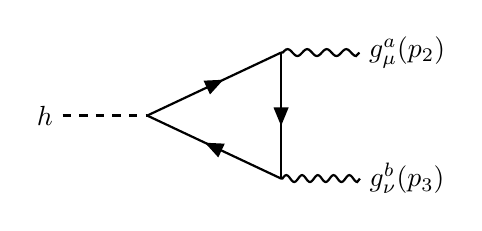
\begin{tikzpicture}[baseline=(current bounding box.center)]
  \begin{feynman}
    % External particles
    \vertex (h)  at (-2.2,0) {$h$};
    \vertex (g1) at (2.4,0.8) {$g_\mu^a(p_2)$};
    \vertex (g2) at (2.4,-0.8) {$g_\nu^b(p_3)$};

    % Triangle vertices
    \vertex (v1) at (-0.9,0);
    \vertex (v2) at (0.8,0.8);
    \vertex (v3) at (0.8,-0.8);

    \diagram*{
      (h) -- [scalar, thick] (v1),

      (v1) -- [fermion, thick] (v2),
      (v2) -- [fermion, thick] (v3),
      (v3) -- [fermion, thick] (v1),

      (v2) -- [boson, thick] (g1),
      (v3) -- [boson, thick] (g2),
    };
  \end{feynman}
\end{tikzpicture}
\quad
+\quad
(u-\text{channel}).
\label{eq:h-to-gg-quark-loop}
\end{equation}
For a particular quark flavour $q$, the scattering amplitude is
\begin{equation}
\begin{aligned}
    i\mathcal M_q^{ab}
    &=
    -\left(-i\frac{y_q}{\sqrt{2}}\right)
    (ig_s)^2
    \int\frac{d^dk}{(2\pi)^d}
    \\
    &\quad\times
    \Tr\left[
        \frac{i(\slashed{k}+m_q)}
        {k^2-m_q^2}
        \gamma^\mu T^a
        \frac{i(\slashed{k}-\slashed{p}_2+m_q)}
        {(k-p_2)^2-m_q^2}
        \gamma^\nu T^b
        \frac{i(\slashed{k}-\slashed{p}_1+m_q)}
        {(k-p_1)^2-m_q^2}
    \right]
    \epsilon_\mu^*(p_2)\epsilon_\nu^*(p_3)
    \\
    &\quad+
    \left(
        p_2,\mu,a\leftrightarrow p_3,\nu,b
    \right)\\
    &=i\frac{y_qg_s^2}{\sqrt{2}}T_F\delta^{ab}
    \epsilon_\mu^*(p_2)\epsilon_\nu^*(p_3)\,8m_q
    \left[
        F_q^{\mu\nu}(p_1,p_2)
        +F_q^{\nu\mu}(p_1,p_3)
    \right],
\end{aligned}
\end{equation}
where $
y_q=\frac{\sqrt2\,m_q}{v}
=2\sqrt{\lambda}\,\frac{m_q}{m_h}
$, and $F_q^{\mu\nu}$ is defined to include the factor of $i$ below, so that it is real for the top-quark loop. Since $y_q\propto m_q$ and $m_b,m_c,m_s,m_d,m_u\ll m_h$, the dominant contribution comes from the top-quark loop. The complete amplitude is obtained by summing over quark flavours. Now, we evaluate the loop integral. The trace can be simplified as
\begin{equation}
\begin{aligned}
&\Tr\left[
        \frac{i(\slashed{k}+m_q)}
        {k^2-m_q^2}
        \gamma^\mu
        \frac{i(\slashed{k}-\slashed{p}_2+m_q)}
        {(k-p_2)^2-m_q^2}
        \gamma^\nu
        \frac{i(\slashed{k}-\slashed{p}_1+m_q)}
        {(k-p_1)^2-m_q^2}
    \right]
\\[2mm]
&=
-\frac{4im_q}{(k^2-m_q^2)[(k-p_2)^2-m_q^2][(k-p_1)^2-m_q^2]}
\Big[
k^\mu(k-p_2)^\nu
+k^\nu(k-p_2)^\mu
-k\cdot(k-p_2)\eta^{\mu\nu}
\\
&\qquad
+k^\mu(k-p_1)^\nu
-k^\nu(k-p_1)^\mu
+k\cdot(k-p_1)\eta^{\mu\nu}
+(k-p_2)^\mu(k-p_1)^\nu
+(k-p_1)^\mu(k-p_2)^\nu
\\
&\qquad
-(k-p_2)\cdot(k-p_1)\eta^{\mu\nu}
+m_q^2\eta^{\mu\nu}
\Big].
\end{aligned}
\end{equation}
Let
\begin{equation}
    A=k^2-m_q^2,\quad B=(k-p_2)^2-m_q^2,\quad C=(k-p_1)^2-m_q^2.
\end{equation}
Introducing Feynman parameter,
\begin{equation}
    \frac{1}{ABC}
    =
    2\int_0^1dx\int_0^{1-x}dy\,
    \frac{1}{[xA+yB+zC]^3},
    \qquad z=1-x-y,
\end{equation}
the denominator becomes
\begin{equation}
\begin{aligned}
xA+yB+zC
&=
k^2-2k\cdot(yp_2+zp_1)
+yp_2^2+zp_1^2-m_q^2
\\
&=
(k-yp_2-zp_1)^2-\Delta,
\end{aligned}
\end{equation}
where
\begin{equation}
    \Delta
    =
    m_q^2-y(1-y)p_2^2-z(1-z)p_1^2
    +2yz\,p_1\cdot p_2.
\end{equation}
Shifting the loop momentum, $\ell = k - yp_2-zp_1\equiv k - P$, the numerator becomes
\begin{equation}
\begin{aligned}
\mathcal N^{\mu\nu}
={}&
4\ell^\mu\ell^\nu-\ell^2\eta^{\mu\nu}
+4P^\mu P^\nu
-2P^\mu(p_1+p_2)^\nu
-2P^\nu p_2^\mu
\\
&+p_1^\mu p_2^\nu+p_2^\mu p_1^\nu
+\left(
m_q^2-P^2+2P\cdot p_2-p_1\cdot p_2
\right)\eta^{\mu\nu}
\\
&+4\ell^\mu P^\nu+4P^\mu\ell^\nu
-2\ell^\mu(p_1+p_2)^\nu
-2\ell^\nu p_2^\mu
+2\ell\cdot(p_2-P)\eta^{\mu\nu}.
\end{aligned}
\end{equation}
The loop integral becomes
\begin{equation}
\begin{aligned}
F^{\mu\nu}_q(p_1,p_2)
&=
i\int_0^1dx\int_0^{1-x}dy
\int\frac{d^d\ell}{(2\pi)^d}
\frac{\mathcal N^{\mu\nu}(\ell,P)}
     {(\ell^2-\Delta)^3}.
\end{aligned}
\end{equation}
The terms with an odd number of $\ell$ in the numerator vanish, and $\ell^\mu \ell^\nu \to \frac{1}{d}\eta^{\mu\nu}\ell^2$, which gives
\begin{equation}
\begin{aligned}
\mathcal N^{\mu\nu}
\longrightarrow{}&
\left(\frac{4}{d}-1\right)\ell^2\eta^{\mu\nu}
+4P^\mu P^\nu
-2P^\mu(p_1+p_2)^\nu
-2P^\nu p_2^\mu
\\
&+p_1^\mu p_2^\nu+p_2^\mu p_1^\nu
+\left(
m_q^2-P^2+2P\cdot p_2-p_1\cdot p_2
\right)\eta^{\mu\nu}.
\end{aligned}
\end{equation}
Then, using dimensional regularisation expanding around $d=4-\epsilon$, we find
\begin{equation}
\begin{aligned}
F_q^{\mu\nu}(p_1,p_2)
=
\frac{-1}{32\pi^2}
\int_0^1dx\int_0^{1-x}dy\,
\frac{1}{m_q^2-xz\,m_h^2}
\Bigg[
&m_h^2\left(\frac12-2xz\right)\eta^{\mu\nu}
\\
&-2z(2z-1)p_1^\mu p_1^\nu
+4y(1-y)p_2^\mu p_2^\nu
\\
&-\left(4yz-2z+1\right)p_1^\mu p_2^\nu
\\
&-\left(4yz-2y-2z+1\right)p_2^\mu p_1^\nu
\Bigg].
\end{aligned}
\end{equation}

Contracting with the on-shell gluon polarisations, it follows that
\begin{equation}
\begin{aligned}
&\epsilon_\mu^*(p_2)\epsilon_\nu^*(p_3)
p_1^\mu p_1^\nu
=
\epsilon_\mu^*(p_2)\epsilon_\nu^*(p_3)
p_1^\mu p_2^\nu
\\
&\qquad=
\bigl[\epsilon^*(p_2)\cdot p_3\bigr]
\bigl[\epsilon^*(p_3)\cdot p_2\bigr],
\end{aligned}
\end{equation}
while all terms proportional to $p_2^\mu$ vanish. Therefore,
\begin{equation}
\begin{aligned}
&\epsilon_\mu^*(p_2)\epsilon_\nu^*(p_3)
F_t^{\mu\nu}(p_1,p_2)
\\
&\quad=
-\frac{1}{32\pi^2}
\int_0^1dx\int_0^{1-x}dy\,
\frac{1-4xz}{m_t^2-xz\,m_h^2}
\\
&\qquad\quad\times
\left[
\frac{m_h^2}{2}\,
\epsilon^*(p_2)\cdot\epsilon^*(p_3)
-
\bigl(\epsilon^*(p_2)\cdot p_3\bigr)
\bigl(\epsilon^*(p_3)\cdot p_2\bigr)
\right].
\end{aligned}
\end{equation}
The crossed orientation gives the same result after relabelling the Feynman parameters. Adding the two orientations gives
\begin{equation}
\begin{aligned}
&\epsilon_\mu^*(p_2)\epsilon_\nu^*(p_3)
\left[
F_t^{\mu\nu}(p_1,p_2)+F_t^{\nu\mu}(p_1,p_3)
\right]
\\
&\quad=
-\frac{1}{16\pi^2}
\left[
\frac{m_h^2}{2}\,
\epsilon^*(p_2)\cdot\epsilon^*(p_3)
-
\bigl(\epsilon^*(p_2)\cdot p_3\bigr)
\bigl(\epsilon^*(p_3)\cdot p_2\bigr)
\right]
\\
&\qquad\quad\times
\int_0^1dx\int_0^{1-x}dy\,
\frac{1-4x(1-x-y)}
{m_t^2-m_h^2x(1-x-y)}.
\end{aligned}
\end{equation}
Evaluating the integral gives
\begin{equation}
\begin{aligned}
&\int_0^1dx\int_0^{1-x}dy\,
\frac{1-4x(1-x-y)}
{m_t^2-m_h^2x(1-x-y)}
\\
&\qquad=
\frac{2}{m_h^2}
\left[
1+\left(1-\frac{4m_t^2}{m_h^2}\right)
\arcsin^2\left(\frac{m_h}{2m_t}\right)
\right].
\end{aligned}
\end{equation}
Thus, the top-loop amplitude becomes
\begin{equation}
\begin{aligned}
i\mathcal M_t^{ab}
={}&
-i\frac{y_tg_s^2m_tT_F}{2\sqrt{2}\pi^2}\,
\delta^{ab}
\left[
1+\left(1-\frac{4m_t^2}{m_h^2}\right)
\arcsin^2\left(\frac{m_h}{2m_t}\right)
\right]
\\
&\times
\epsilon_\mu^*(p_2)\epsilon_\nu^*(p_3)
\left[
\eta^{\mu\nu}
-\frac{2}{m_h^2}p_3^\mu p_2^\nu
\right].
\label{eq:iM_t}
\end{aligned}
\end{equation}
Using
\begin{equation}
\sum_{\mathrm{pols.}}
\epsilon_\mu^*(p)\epsilon_\nu(p)
=-\eta_{\mu\nu},
\qquad
\sum_{a,b}\delta^{ab}\delta^{ab}=N_c^2-1=8,
\qquad
T_F=\frac12,
\end{equation}
and
\begin{equation}
\left[
\eta^{\mu\nu}-\frac{2}{m_h^2}p_3^\mu p_2^\nu
\right]
\left[
\eta_{\mu\nu}-\frac{2}{m_h^2}p_{3\mu}p_{2\nu}
\right]
=2,
\end{equation}
we finally obtain
\begin{equation}
\begin{aligned}
\sum_{\mathrm{pols./colours}}|\mathcal M_t|^2
={}&
\frac{m_t^2y_t^2g_s^4}{2\pi^4}
\left[
1+\left(1-\frac{4m_t^2}{m_h^2}\right)
\arcsin^2\left(\frac{m_h}{2m_t}\right)
\right]^2.
\end{aligned}
\end{equation}
Here we have neglected the contributions from the remaining quarks.

Plugging into \eqref{eq:decayrate}, we find
\begin{equation}
\begin{aligned}
\boxed{
    \Gamma(H \to gg) = \frac{\lambda g_s^4 m_t^4}{16\pi^5m_h^3}\left[
1+\left(1-\frac{4m_t^2}{m_h^2}\right)
\arcsin^2\left(\frac{m_h}{2m_t}\right)
\right]^2,}
\end{aligned}
\end{equation}
where a factor of $1/2$ is added since the outgoing gluon states are identical.
This gives a numerical value of
\begin{equation}
    \boxed{
\Gamma(H\to gg)
\simeq 1.97\times10^{-4}\ \mathrm{GeV}
=0.197\ \mathrm{MeV}.
}
\end{equation}

Now we turn to the computation of $H \to \gamma\gamma$. Similarly to the gluon case, there is no tree-level contribution to the process. The dominant quark-loop contribution comes from the top-quark loop, just as for the gluon case. On top of that, there is also a contribution from a $W$-boson loop. Therefore, our job is to compute the following diagrams
% Top-quark loop and crossed diagram
\begin{equation}
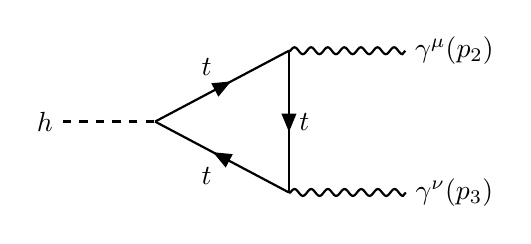
\begin{tikzpicture}[baseline=(current bounding box.center)]
  \begin{feynman}
    \vertex (h)  at (-2.2,0) {$h$};
    \vertex (v1) at (-0.8,0);
    \vertex (v2) at (0.9,0.9);
    \vertex (v3) at (0.9,-0.9);
    \vertex (g1) at (3.0,0.9) {$\gamma^\mu(p_2)$};
    \vertex (g2) at (3.0,-0.9) {$\gamma^\nu(p_3)$};

    \diagram*{
      (h)  -- [scalar, thick] (v1),
      (v1) -- [fermion, thick, edge label=$t$] (v2),
      (v2) -- [fermion, thick, edge label=$t$] (v3),
      (v3) -- [fermion, thick, edge label=$t$] (v1),
      (v2) -- [photon, thick] (g1),
      (v3) -- [photon, thick] (g2),
    };
  \end{feynman}
\end{tikzpicture}
\quad+\quad
\left(p_2,\mu\leftrightarrow p_3,\nu\right)
\quad=\quad i\mathcal M_t^\gamma.
\end{equation}

% W-boson loop and crossed diagram
\begin{equation}
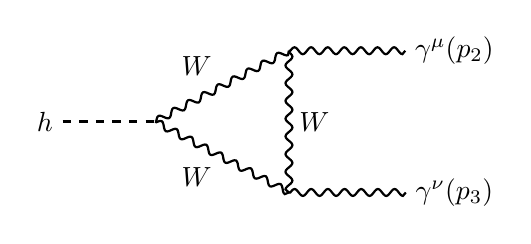
\begin{tikzpicture}[baseline=(current bounding box.center)]
  \begin{feynman}
    \vertex (h)  at (-2.2,0) {$h$};
    \vertex (v1) at (-0.8,0);
    \vertex (v2) at (0.9,0.9);
    \vertex (v3) at (0.9,-0.9);
    \vertex (g1) at (3.0,0.9) {$\gamma^\mu(p_2)$};
    \vertex (g2) at (3.0,-0.9) {$\gamma^\nu(p_3)$};

    \diagram*{
      (h)  -- [scalar, thick] (v1),
      (v1) -- [boson, thick, edge label=$W$] (v2),
      (v2) -- [boson, thick, edge label=$W$] (v3),
      (v1) -- [boson, thick, edge label'=$W$] (v3),
      (v2) -- [photon, thick] (g1),
      (v3) -- [photon, thick] (g2),
    };
  \end{feynman}
\end{tikzpicture}
\quad+\quad
\left(p_2,\mu\leftrightarrow p_3,\nu\right)
\quad=\quad i\mathcal M_W,
\end{equation}
\begin{equation}
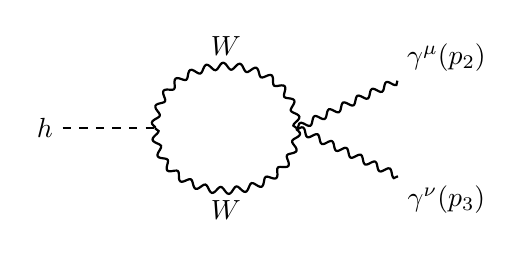
\begin{tikzpicture}[baseline=(current bounding box.center)]
  \begin{feynman}
    \vertex (h)  at (-2.3,0) {$h$};
    \vertex (v1) at (-0.9,0);
    \vertex (v2) at (0.9,0);
    \vertex (g1) at (2.8,0.9)  {$\gamma^\mu(p_2)$};
    \vertex (g2) at (2.8,-0.9) {$\gamma^\nu(p_3)$};

    \diagram*{
      (h) -- [scalar, thick] (v1),

      (v1) -- [
        boson,
        thick,
        half left,
        looseness=1.5,
        edge label=$W$
      ] (v2),

      (v2) -- [
        boson,
        thick,
        half left,
        looseness=1.5,
        edge label=$W$
      ] (v1),

      (v2) -- [photon, thick] (g1),
      (v2) -- [photon, thick] (g2),
    };
  \end{feynman}
\end{tikzpicture}
\quad = \quad i\mathcal M_{W,4}^{\mu\nu}.
\label{eq:h-to-gamma-gamma-W-seagull}
\end{equation}
The relevant interactions are
\begin{equation}
\begin{aligned}
    \mathcal{L}_\mathrm{int} =&-ie[F^{\mu\nu}W^+_\mu W^-_\nu-(\partial_\mu W^+_\nu - \partial_\nu W^+_\mu)A^\mu (W^-)^\nu+(\partial_\mu W^-_\nu - \partial_\nu W^-_\mu)A^\mu (W^+)^\nu]\\ &+ 2\frac{h}{v}m_W^2W_\mu^+ W_\nu ^- +e^2(A^\mu W_\mu^+A^\nu W_\nu^- - A_\mu^2W_\nu^+(W^-)^\nu)- \frac{y_t}{\sqrt{2}}h\bar t t + \frac{2e}{3}A_\mu \bar t \gamma^\mu t,
\end{aligned}
\end{equation}
where the first three interactions are given by the diagrams
% Higgs--W^+--W^- interaction
\begin{equation}
\begin{tikzpicture}[baseline=(v.center)]
  \begin{feynman}
    \vertex (v)  at (0,0);
    \vertex (h)  at (0,1.0)       {$h$};
    \vertex (wp) at (-1.4,-0.8)   {$W^{+\mu}$};
    \vertex (wm) at (1.4,-0.8)    {$W^{-\nu}$};

    \diagram*{
      (h)  -- [scalar, thick] (v),
      (wp) -- [boson, thick]  (v),
      (wm) -- [boson, thick]  (v),
    };
  \end{feynman}
\end{tikzpicture}
\quad = \quad
i\frac{e\,m_W}{\sin\theta_w}\eta^{\mu\nu},
\label{eq:hWW-interaction}
\end{equation}

% Photon--W^+--W^- interaction
\begin{equation}
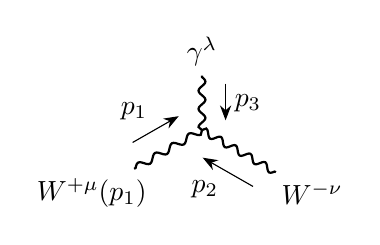
\begin{tikzpicture}[baseline=(v.center)]
  \begin{feynman}
    \vertex (v)  at (0,0);
    \vertex (a)  at (0,1.0)       {$\gamma^\lambda$};
    \vertex (wp) at (-1.4,-0.8)   {$W^{+\mu}(p_1)$};
    \vertex (wm) at (1.4,-0.8)    {$W^{-\nu}$};

    \diagram*{
      (a)  -- [photon, thick, momentum = $p_3$] (v),
      (wp) -- [boson, thick, momentum = $p_1$]  (v),
      (wm) -- [boson, thick, momentum = $p_2$]  (v),
    };
  \end{feynman}
\end{tikzpicture}
\quad = \quad
-ie
\begin{aligned}[t]
\Big[
&\eta^{\mu\nu}(p_1-p_2)^\lambda
+\eta^{\nu\lambda}(p_2-p_3)^\mu
\\
&+\eta^{\lambda\mu}(p_3-p_1)^\nu
\Big],
\end{aligned}
\label{eq:gammaWW-interaction}
\end{equation}
% Photon--photon--W^+--W^- interaction
\begin{equation}
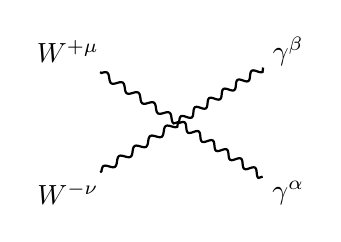
\begin{tikzpicture}[baseline=(v.center)]
  \begin{feynman}
    \vertex (v)  at (0,0);
    \vertex (wp) at (-1.4,0.9)  {$W^{+\mu}$};
    \vertex (wm) at (-1.4,-0.9) {$W^{-\nu}$};
    \vertex (a2) at (1.4,0.9)   {$\gamma^\beta$};
    \vertex (a1) at (1.4,-0.9)  {$\gamma^\alpha$};

    \diagram*{
      (wp) -- [boson, thick] (v),
      (wm) -- [boson, thick] (v),
      (v)  -- [photon, thick] (a2),
      (v)  -- [photon, thick] (a1),
    };
  \end{feynman}
\end{tikzpicture}
\quad = \quad
ie^2
\begin{aligned}[t]
\Big[
&\eta^{\alpha\mu}\eta^{\beta\nu}
+\eta^{\alpha\nu}\eta^{\beta\mu}
-2\eta^{\alpha\beta}\eta^{\mu\nu}
\Big].
\end{aligned}
\label{eq:gammagammaWW-interaction}
\end{equation}
and the last two are Yukawa and QED interactions. Note that $i\mathcal{M}_t^\gamma$ is almost identical to $i\mathcal{M}_t$, but now the colour trace gives $N_c=3$ and $g_s \to 2e/3$. Therefore, we can read off from \eqref{eq:iM_t},
\begin{equation}
\begin{aligned}
i\mathcal M_t^{\gamma}
={}&
-i\frac{2y_te^2m_t}{3\sqrt{2}\pi^2}\,
\left[
1+\left(1-\frac{4m_t^2}{m_h^2}\right)
\arcsin^2\left(\frac{m_h}{2m_t}\right)
\right]
\\
&\times
\epsilon_\mu^*(p_2)\epsilon_\nu^*(p_3)
\left[
\eta^{\mu\nu}
-\frac{2}{m_h^2}p_3^\mu p_2^\nu
\right].
\label{eq:iM_tgamma}
\end{aligned}
\end{equation}
Although rather tedious, we can also read off the $W$ bosons loop diagram from the Feynman rules (or one can easily obtain the expression using the power of AI).
In unitary gauge, the $W$-boson propagator is
\begin{equation}
    D_W^{\alpha\beta}(q)
    =
    \frac{-iP^{\alpha\beta}(q)}
         {q^2-m_W^2},
    \qquad
    P^{\alpha\beta}(q)
    \equiv
    \eta^{\alpha\beta}
    -\frac{q^\alpha q^\beta}{m_W^2}.
\end{equation}
It is useful to define the momentum-dependent part of the
$\gamma W^+W^-$ vertex by
\begin{equation}
\begin{aligned}
\Gamma^{\lambda\alpha\beta}(q,r,s)
={}&
\eta^{\alpha\beta}(r-s)^\lambda
+\eta^{\beta\lambda}(s-q)^\alpha
+\eta^{\lambda\alpha}(q-r)^\beta,
\end{aligned}
\end{equation}
so that the vertex is $-ie\Gamma^{\lambda\alpha\beta}(q,r,s)$.

The triangle diagram and its crossed photon ordering together give
\begin{equation}
\begin{aligned}
i\mathcal M_{W}
={}&
\frac{e^3m_W}{\sin\theta_w}
\epsilon_\mu^*(p_2)\epsilon_\nu^*(p_3)
\int\frac{d^dk}{(2\pi)^d}
\Bigg[
\frac{\mathcal N^{\mu\nu}(k;p_2,p_3)}
     {(k^2-m_W^2)
      [(k-p_2)^2-m_W^2]
      [(k-p_1)^2-m_W^2]}
\\
&\hspace{4.2cm}
+
\frac{\mathcal N^{\nu\mu}(k;p_3,p_2)}
     {(k^2-m_W^2)
      [(k-p_3)^2-m_W^2]
      [(k-p_1)^2-m_W^2]}
\Bigg],
\end{aligned}
\end{equation}
where
\begin{equation}
\begin{aligned}
\mathcal N^{\mu\nu}(k;p_2,p_3)
={}&
\eta^{\alpha\rho}
P_{\alpha\beta}(k)
\Gamma^{\mu\beta\gamma}
    (-p_2,k,p_2-k)
\\
&\times
P_{\gamma\delta}(k-p_2)
\Gamma^{\nu\delta\sigma}
    (-p_3,k-p_2,p_1-k)
P_{\sigma\rho}(k-p_1).
\end{aligned}
\end{equation}
The quartic $\gamma\gamma W^+W^-$ bubble diagram
must also be included. Define
\begin{equation}
    Q^{\mu\nu\beta\sigma}
    =
    \eta^{\mu\beta}\eta^{\nu\sigma}
    +\eta^{\mu\sigma}\eta^{\nu\beta}
    -2\eta^{\mu\nu}\eta^{\beta\sigma},
\end{equation}
so that the quartic vertex is $ie^2Q^{\mu\nu\beta\sigma}$.
Its contribution is
\begin{equation}
\begin{aligned}
i\mathcal M_{W,4}
={}&
\frac{e^3m_W}{\sin\theta_w}
\epsilon_\mu^*(p_2)\epsilon_\nu^*(p_3)
\int\frac{d^dk}{(2\pi)^d}
\frac{
\eta^{\alpha\rho}
P_{\alpha\beta}(k)
Q^{\mu\nu\beta\sigma}
P_{\sigma\rho}(k-p_1)
}{
(k^2-m_W^2)[(k-p_1)^2-m_W^2]
}.
\end{aligned}
\end{equation}

Now, we shall evaluate the two diagrams.
Introduce Feynman parameters,
\begin{equation}
\begin{aligned}
\frac{1}{D_0D_2D_1}
&=
2\int_0^1dx\int_0^{1-x}dy\,
\frac{1}{[xD_0+yD_2+zD_1]^3},
\\
\frac{1}{D_0D_3D_1}
&=
2\int_0^1dx\int_0^{1-x}dy\,
\frac{1}{[xD_0+yD_3+zD_1]^3},
\qquad
z=1-x-y,
\end{aligned}
\end{equation}
where
\begin{equation}
\begin{aligned}
D_0&=k^2-m_W^2,
&
D_1&=(k-p_1)^2-m_W^2,
\\
D_2&=(k-p_2)^2-m_W^2,
&
D_3&=(k-p_3)^2-m_W^2.
\end{aligned}
\end{equation}
For the first and crossed orientations, respectively, make the shifts
\begin{equation}
\begin{aligned}
    \ell&=k-yp_2-zp_1,
&
    \ell&=k-yp_3-zp_1.
\end{aligned}
\end{equation}
Using
\begin{equation}
    p_1=p_2+p_3,
    \qquad
    p_1^2=m_h^2,
    \qquad
    p_2^2=p_3^2=0,
\end{equation}
both denominators reduce to
\begin{equation}
    xD_0+yD_{2,3}+zD_1
    =
    \ell^2-\Delta,
    \qquad
    \Delta=m_W^2-xz\,m_h^2.
\end{equation}
Therefore, the two triangle orientations together become
\begin{equation}
\begin{aligned}
i\mathcal M_{W}
={}&
2\frac{e^3m_W}{\sin\theta_w}
\epsilon_\mu^*(p_2)\epsilon_\nu^*(p_3)
\int_0^1dx\int_0^{1-x}dy
\int\frac{d^d\ell}{(2\pi)^d}
\\
&\times
\frac{
\mathcal N^{\mu\nu}
\bigl(\ell+yp_2+zp_1;p_2,p_3\bigr)
+
\mathcal N^{\nu\mu}
\bigl(\ell+yp_3+zp_1;p_3,p_2\bigr)
}{
(\ell^2-\Delta)^3
}.
\end{aligned}
\end{equation}
For convenience, define the combined numerator
\begin{equation}
\begin{aligned}
\widetilde{\mathcal N}^{\mu\nu}(\ell;x,y)
\equiv{}&
\mathcal N^{\mu\nu}
\bigl(\ell+yp_2+zp_1;p_2,p_3\bigr)
\\
&+
\mathcal N^{\nu\mu}
\bigl(\ell+yp_3+zp_1;p_3,p_2\bigr).
\end{aligned}
\end{equation}
Thus,
\begin{equation}
\begin{aligned}
i\mathcal M_{W}
={}&
2\frac{e^3m_W}{\sin\theta_w}
\epsilon_\mu^*(p_2)\epsilon_\nu^*(p_3)
\int_0^1dx\int_0^{1-x}dy
\int\frac{d^d\ell}{(2\pi)^d}
\frac{
\widetilde{\mathcal N}^{\mu\nu}(\ell;x,y)
}{
(\ell^2-\Delta)^3
}.
\end{aligned}
\end{equation}
To ensure convergence we should include the four-point diagram before carrying out the loop integral.
The terms with odd $l$ in the numerator vanishes and $l^\mu l^\nu \to \frac{1}{d}\eta^{\mu\nu}l^2$, the $l^4$ term in $i\mathcal{M}_{W,4}$ becomes
\begin{equation}
\begin{aligned}
\ell^\mu\ell^\nu\ell^\rho\ell^\sigma
\longrightarrow
\frac{\ell^4}{d(d+2)}
\Big(
&\eta^{\mu\nu}\eta^{\rho\sigma}
+\eta^{\mu\rho}\eta^{\nu\sigma}
+\eta^{\mu\sigma}\eta^{\nu\rho}
\Big).
\end{aligned}
\end{equation}
After some long and cumbersome algebra, one would find
\begin{equation}
\begin{aligned}
i\mathcal M_W+i\mathcal M_{W,4}
={}&
i\frac{e^3}
{16\pi^2m_W\sin\theta_w}
\epsilon_\mu^*(p_2)\epsilon_\nu^*(p_3)
\left[
(p_2\cdot p_3)\eta^{\mu\nu}
-p_3^\mu p_2^\nu
\right]
\\
&\times
\left[
2+
12m_W^2
\int_0^1dx\int_0^{1-x}dy\,
\frac{1-2xz}{m_W^2-m_h^2xz}
\right].
\end{aligned}
\end{equation}
The integral can be evaluated, which gives
\begin{equation}
\begin{aligned}
\int_0^1dx\int_0^{1-x}dy\,
\frac{1-2xz}{m_W^2-m_h^2xz}
=
\frac{1}{m_h^2}
\left[
1+\left(2-\frac{4m_W^2}{m_h^2}\right)\arcsin^2\left(\frac{m_h}{2m_W}\right)
\right].
\end{aligned}
\end{equation}
Finally, we end up with
\begin{equation}
\begin{aligned}
i\mathcal M_W + i\mathcal M_{W,4}
={}&
i\frac{e^3}
{16\pi^2m_W\sin\theta_w}
\Bigg[
2+\frac{12m_W^2}{m_h^2}
+\frac{24m_W^2}{m_h^2}
\left(
1-\frac{2m_W^2}{m_h^2}
\right)
\arcsin^2\left(\frac{m_h}{2m_W}\right)
\Bigg]
\\
&\times
\epsilon_\mu^*(p_2)\epsilon_\nu^*(p_3)
\left[
(p_2\cdot p_3)\eta^{\mu\nu}
-p_3^\mu p_2^\nu
\right].
\end{aligned}
\end{equation}

To combine the top and $W$ contributions, define
\begin{equation}
\begin{aligned}
\mathcal F_t
={}&
\frac{32m_t^2}{3m_h^2}
\left[
1+\left(1-\frac{4m_t^2}{m_h^2}\right)
\arcsin^2\left(\frac{m_h}{2m_t}\right)
\right],
\\
\mathcal F_W
={}&
2+\frac{12m_W^2}{m_h^2}
+\frac{24m_W^2}{m_h^2}
\left(1-\frac{2m_W^2}{m_h^2}\right)
\arcsin^2\left(\frac{m_h}{2m_W}\right).
\end{aligned}
\end{equation}
Using $y_t=\sqrt{2}m_t/v$ and
$m_W=e v/(2\sin\theta_w)$, the total amplitude is
\begin{equation}
\begin{aligned}
i\mathcal M_{\gamma\gamma}
={}&
i\frac{e^3}{16\pi^2m_W\sin\theta_w}
(\mathcal F_W-\mathcal F_t)
\epsilon_\mu^*(p_2)\epsilon_\nu^*(p_3)
\left[
(p_2\cdot p_3)\eta^{\mu\nu}
-p_3^\mu p_2^\nu
\right].
\end{aligned}
\end{equation}
Thus, using $p_2\cdot p_3=m_h^2/2$, the polarization sum gives
\begin{equation}
\begin{aligned}
\sum_{\mathrm{pols.}}|\mathcal M_{\gamma\gamma}|^2
&=
\frac{e^6}{256\pi^4m_W^2\sin^2\theta_w}
(\mathcal F_W-\mathcal F_t)^2
\left[
(p_2\cdot p_3)\eta^{\mu\nu}-p_3^\mu p_2^\nu
\right]
\left[
(p_2\cdot p_3)\eta_{\mu\nu}-p_{3\mu}p_{2\nu}
\right]
\\
&=
\frac{e^6m_h^4}{512\pi^4m_W^2\sin^2\theta_w}
(\mathcal F_W-\mathcal F_t)^2.
\end{aligned}
\end{equation}
The two photons are identical, so the two-body phase space includes a factor
of $1/2!$. Therefore,
\begin{equation}
\boxed{
\Gamma(H\to\gamma\gamma)
=
\frac{e^6m_h^3}{16384\pi^5m_W^2\sin^2\theta_w}
(\mathcal F_W-\mathcal F_t)^2
=
\frac{\alpha^2m_h^3}{256\pi^3v^2}
(\mathcal F_W-\mathcal F_t)^2.
}
\end{equation}
Using
\begin{equation}
\begin{aligned}
m_h&=125.20~\mathrm{GeV},
&m_t&=172.56~\mathrm{GeV},
&m_W&=80.377~\mathrm{GeV},
\\
v&=246.22~\mathrm{GeV},
&\alpha^{-1}&=137.036,
\end{aligned}
\end{equation}
we find
\begin{equation}
\mathcal F_t\simeq1.836,
\qquad
\mathcal F_W\simeq8.331,
\end{equation}
and hence
\begin{equation}
\boxed{
\Gamma(H\to\gamma\gamma)
\simeq9.16\times10^{-6}~\mathrm{GeV}
=9.16~\mathrm{keV}.
}
\end{equation}

Finally, the three branching ratios are compared in
Fig.~\ref{fig:higgs-branching-ratios}. The denominator is the full
Standard Model Higgs width, rather than only the sum of the three channels
calculated above. The broad mass scan is taken from the LHC Higgs Cross
Section Working Group report CERN-2011-002, while the precise values quoted
below at $m_h=125.2~\mathrm{GeV}$ use the newer Yellow Report 4 table.
\begin{figure}[t]
    \centering
    
\includegraphics{schwartz-problem-29-3-branching-ratios.png}
    \caption{
        Standard Model branching ratios for $H\to b\bar b$, $H\to gg$,
        and $H\to\gamma\gamma$ for $90\leq m_h\leq1000~\mathrm{GeV}$.
        The values are taken from Tables 26--29 of CERN-2011-002 and use
        the full Standard Model decay width. Above approximately
        $500~\mathrm{GeV}$, the on-shell Higgs treatment used in these
        tables should be interpreted with care.
    }
    \label{fig:higgs-branching-ratios}
\end{figure}
At $m_h=125.2~\mathrm{GeV}$, the corresponding values are
\begin{equation}
    \operatorname{BR}(H\to b\bar b)=0.5792,
    \qquad
    \operatorname{BR}(H\to gg)=0.08172,
    \qquad
    \operatorname{BR}(H\to\gamma\gamma)=0.002270.
\end{equation}
\clearpage

\end{solution}

\subsection[Problem 29.6: Phases in the PMNS matrix]{Problem 29.6: Phases in the PMNS Matrix}

Show that with general Dirac and Majorana mass matrices, there are three phases
in the PMNS matrix, while if the mass matrix is purely Dirac, there is only one.
How many phases are there if the masses are purely Majorana?

\begin{solution}
A general \(3\times3\) unitary PMNS matrix contains three mixing angles and six phases. The three charged-lepton fields can always be rephased, removing three phases. If the neutrinos are Dirac particles, the three neutrino mass eigenstates can also be rephased. However, one common rephasing of all charged leptons and neutrinos leaves the PMNS matrix unchanged, so only \(3+3-1=5\) phases can be removed, leaving one physical phase. If any Majorana mass is present, the neutrino mass eigenstates are generically Majorana and cannot be continuously rephased, since the Majorana condition \(N_i^c=N_i\) is preserved only by the discrete transformation \(N_i\to\pm N_i\). Consequently, only the three charged-lepton rephasings are available, leaving \(6-3=3\) physical phases. The same reasoning applies to purely Majorana masses. Thus the PMNS matrix contains one physical phase for purely Dirac neutrinos and three physical phases for either Dirac-plus-Majorana or purely Majorana neutrinos.
\end{solution}

\subsection[Problem 29.7: Neutrino oscillations]{Problem 29.7: Neutrino Oscillations}

Neutrino oscillations.

\begin{enumerate}
  \item Neutrinos are produced in the Sun predominantly through the reaction
  $p+p+e^-\to d+\nu_e$. What is the momentum of the neutrinos produced this
  way?

  \item Consider a two-neutrino flavour system. The mass eigenstates evolve in
  time as
  \begin{align}
    |\nu_1\rangle
      &=e^{-iE_1t}\bigl(\cos\theta\,|\nu_e\rangle
        +\sin\theta\,|\nu_\mu\rangle\bigr),\\
    |\nu_2\rangle
      &=e^{-iE_2t}\bigl(-\sin\theta\,|\nu_e\rangle
        +\cos\theta\,|\nu_\mu\rangle\bigr),
  \end{align}
  where $\theta$ is the mixing angle. Show that the probability of finding a
  solar neutrino as an electron neutrino after a time $T$ is given by
  \begin{equation}
    P=1-\sin^2(2\theta)\sin^2\!\left(\frac{(E_2-E_1)T}{2}\right).
    \label{eq:b}
  \end{equation}

  \item Take the high-energy limit $E\gg m_\nu$ to show that the
  probability of finding a solar neutrino with energy $E$ as an electron
  neutrino at a distance $L$ is given by
  \begin{equation}
    P=1-\sin^2(2\theta)\sin^2\!\left(\frac{\Delta m^2L}{4E}\right).
  \end{equation}

  \item How far should you put your detector from a reactor producing
  $\sim4\,\mathrm{MeV}$ neutrinos assuming
  $\Delta m^2=7.5\times10^{-5}\,\mathrm{eV}^2$ to see the largest effect?
\end{enumerate}

\begin{solution}
    Neglecting the thermal kinetic energy of the particles, the four-momentum before reaction is given by $k^\mu = (2m_p + m_e = s, 0 )$. By four-momentum conservation $p_{\nu_e} + p_d = k$, we have
    \begin{equation}
        p_d^2 = m_d^2 = (k-p_{\nu_e})^2 = s+ m_{\nu_e}^2 -2\sqrt{s}E_{\nu_e} \implies E_{\nu_e} = \frac{s+m_{\nu_e}^2 -m_d^2}{s\sqrt{s}} = \sqrt{m_d^2 +|\mathbf{p}_{\nu_e}|^2}.
    \end{equation}
    Therefore, we find
    \begin{equation}
        |\mathbf{p}_{\nu_e}| \approx 1.44 ~\mathrm{MeV}.
    \end{equation}

    The solar neutrino is produced as an electron neutrino. That is, at $t=0$,
    \begin{equation}
        \ket{\nu;t=0} = \ket{\nu_e} = \cos\theta\ket{\nu_1} - \sin\theta \ket{\nu_2}.
    \end{equation}
    Carrying out a standard QM calculation, it is easy to obtain \eqref{eq:b}.

    In the high-energy limit,
    \begin{equation}
        E_1  \approx |\mathbf{p}|\left(1-\frac{m_1^2}{2|\mathbf{p}|^2}\right) \implies -\Delta E \approx \frac{2\Delta m^2}{2|\mathbf{p}|} \approx \frac{2\Delta m^2}{2E}.
    \end{equation}
    In natural units, $T \approx L$, and hence, we find the desired equation.

    The maxima occur at
    \begin{equation}
        L_n = \frac{2\pi E}{\Delta m^2}(2n+1), \quad L_0 \approx 66 ~\mathrm{km}.
    \end{equation}
\end{solution}

\subsection[Problem 29.8: Integrating out right-handed neutrinos]{Problem 29.8: Integrating Out Right-Handed Neutrinos}

Show that when you integrate out the right-handed neutrinos in Eq.~(29.63), a
dimension-5 operator like that in Eq.~(29.65) results. What is the exact
relationship between $M_{ij}$ and $\widetilde M_{ij}$?

\begin{solution}
    The relevant Lagrangian for the right-handed neutrino is
    \begin{equation}
        \mathcal{L} =i\bar\nu^i_R(\slashed{\partial}-ig'Y_\nu \slashed{B})\nu_R^i - Y_{ij}^\nu\bar L^i\tilde{H}\nu_R^j - iM_{ij}(\nu_R^i)^c\nu_R^j,
    \end{equation}
    where the hypercharge $Y_\nu$ vanishes. The equation of motion is given by
    \begin{equation}
        -i(\partial_\mu \nu_R^{i\dagger})\sigma^\mu  - Y_{ji}^{\nu}(\bar L^j \tilde H) -2iM_{ji}(\nu_R^{j})^T\sigma_2 = 0.
    \end{equation}
    At low energy compared to $M_{ij}$, the kinetic term of the right-handed neutrino can be neglected, and we find
    \begin{equation}
        -iM_{ij}(\nu_R^j)^T\sigma_2 = -\frac{1}{2}Y^\nu_{ji}(\bar L^j\tilde H), \quad M_{ij}\nu_R^j = -\frac{1}{2}i\sigma_2Y^\nu_{ij}(\bar L^j\tilde H)^T,
    \end{equation}
    where we have used $M_{ij} = M_{ji}$.
    Therefore, we find
    \begin{equation}
        -iM_{ij}(\nu_R^i)^c\nu_R^j = \frac{i}{4}Y_{ij}^\nu M^{-1}_{jk}Y_{kl}^\nu(\bar L^i\tilde H) \sigma_2(\bar L^l\tilde H)^T,
    \end{equation}
    which gives
    \begin{equation}
    \boxed{
        \widetilde M_{il} = - \frac{i}{4}Y_{ij}^\nu M^{-1}_{jk}Y_{kl}^\nu.
        }
    \end{equation}

\end{solution}

\subsection[Problem 29.9: Chiral rotations and the \texorpdfstring{$\theta$}{theta} angle]{Problem 29.9: Chiral Rotations and the Theta Angle}

Show that when multiple generations are rotated, then the $\theta$ angle shifts
by $\arg\det(R^\dagger L)$.

\begin{solution}
For $N$ generations, the chiral rotations are
\begin{equation}
    \psi_R^i\to R^{ij}\psi_R^j,
    \qquad
    \psi_L^i\to L^{ij}\psi_L^j,
\end{equation}
where $R,L\in U(N)$. We decompose
\begin{equation}
    U(N)=SU(N)\times U(1),
\end{equation}
and write
\begin{equation}
    R=e^{ir/N}\widetilde R,
    \qquad
    L=e^{i\ell/N}\widetilde L,
\end{equation}
where
\begin{equation}
    \widetilde R,\widetilde L\in SU(N),
    \qquad
    \det\widetilde R=\det\widetilde L=1.
\end{equation}

Under the $SU(N)$ transformations, the Grassmann measures transform as
\begin{equation}
    \prod_i\mathcal D\psi_R^i
    \to
    (\det\widetilde R)^{-1}
    \prod_i\mathcal D\psi_R^i
    =
    \prod_i\mathcal D\psi_R^i
\end{equation}
and
\begin{equation}
    \prod_i\mathcal D\psi_L^i
    \to
    (\det\widetilde L)^{-1}
    \prod_i\mathcal D\psi_L^i
    =
    \prod_i\mathcal D\psi_L^i.
\end{equation}
The conjugate-field measures are also invariant. Therefore, the $SU(N)$
parts of $R$ and $L$ do not change the complete functional measure. Only the
$U(1)$ parts can shift the $\theta$ angle.

The remaining $U(1)$ transformations are
\begin{equation}
    \psi_R\to e^{ir/N}\psi_R,
    \qquad
    \psi_L\to e^{i\ell/N}\psi_L.
\end{equation}
These can be written as a vector rotation and an axial rotation:
\begin{equation}
    \psi\to e^{i\alpha_V}e^{i\alpha_A\gamma^5}\psi,
\end{equation}
where
\begin{equation}
    \alpha_V=\frac{r+\ell}{2N},
    \qquad
    \alpha_A=\frac{r-\ell}{2N}.
\end{equation}
The vector rotation leaves the functional measure invariant. An axial
rotation by $\alpha_A$ shifts the $\theta$ angle by $-2\alpha_A$ for each
generation. Since there are $N$ generations,
\begin{equation}
    \Delta\theta=-2N\alpha_A
    =-2N\left(\frac{r-\ell}{2N}\right)
    =\ell-r.
\end{equation}

Finally,
\begin{equation}
\begin{aligned}
    \det(R^\dagger L)
    &=(\det R)^*\det L\\
    &=e^{-ir}e^{i\ell}\\
    &=e^{i(\ell-r)}.
\end{aligned}
\end{equation}
Therefore,
\begin{equation}
    \arg\det(R^\dagger L)=\ell-r=\Delta\theta,
\end{equation}
and hence
\begin{equation}
    \boxed{
        \theta\to\theta+\arg\det(R^\dagger L)
    }.
\end{equation}
\end{solution}

\subsection{End of imported solutions}
\end{document}
